\documentclass{subfiles}

\begin{document}
    \subsection*{Versuchsprotokoll} 
        \marginnote{Start 9:20}
        Wir einigen uns auf den Ordnernamen 
        \begin{center}
            \texttt{./Tiwary-Jannack-Folgmann/}
        \end{center}
        und sortieren in Unterordnern \texttt{./i} für $i$ als Versuchsdurchführungsnummer. Als Test nehmen wir die in \ref{fig:TestPulseAndCollect} dargestellten folgenden Parameter auf:
        \begin{figure}[H]
            \centering
            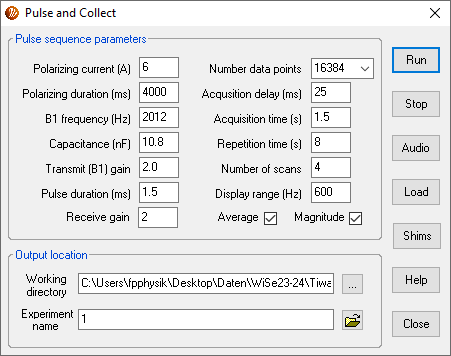
\includegraphics[width=5cm]{Bilddateien/Versuchsbilder/Testaufnahme-Pulse-And-Collect.PNG}
            \caption{Testaufnahme der \enquote{Pulse and Collect} Parameter.}
            \label{fig:TestPulseAndCollect}
        \end{figure}


        \paragraph*{Versuchsteil 3}
            Wir sind uns unsicher, was die Aussage des Rauschens ist. 
\end{document}